\ifgerman{\chapter{Anhang}}{\chapter{Appendix}}
\label{ch:appedix}
\section{Backpropagation Example}

To better understand the backpropagation algorithm mention in \ref{backprop}, consider the following example.

\begin{figure}[!ht]
    \centering
    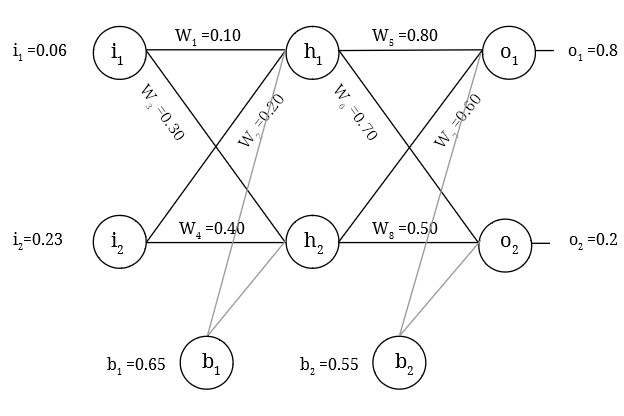
\includegraphics[width=8cm,height=6cm, keepaspectratio]{pics/BackpropExample.jpg}
    \caption{Basic structure of a neural network with weights and bais initialized}
    \label{fig:bakprop}
\end{figure}

The goal of backpropagation is the adjust the weights such that the neural network can correctly map the input to the output. To begin with consider the neural network in the \ref{fig:bakprop} with inputs to the neural network be $i_{1} = 0.06$ and $i_{2} = 0.23$ to which the neural network should output $o_{1}=0.8$ and $o_{2}=0.2$.

In the forward pass, the neural network is feed in the inputs and given the weights and biases in the \ref{fig:bakprop}, it has to predict the output. It has to figure out the output at each hidden layer neuron, i.e $h_{1}$ and $h_{2}$ and squash each output using activation function and do the same at output layer. The activation function in this case is a \textit{logistic function} of which sigmoid activation is a special case.

To calculate the input at $h_{1}$ as $net_{h_{1}}$ we can use \ref{eq:NNformula} as follows,
\begin{align}
    net_{h_{1}} &= W_{1} * i_{1} + W_{2} * i_{2} +b_{1}\\
    net_{h_{1}} &= 0.10 * 0.60 + 0.20 * 0.23 + 0.65 \\
    net_{h_{1}} &= 0.756 \label{eq:endH1}
\end{align}

And to get the output $out_{h_{1}}$ at $h_{1}$ we apply logistic function to \ref{eq:endH1},
\begin{align}
    out_{h_{1}} &= \frac{1}{1+e^{-net_{h_{1}}}}\\
    out_{h_{1}} &=  \frac{1}{1+e^{0.756}}\\
    out_{h_{1}} &= 0.680 \label{eq:outH1}
\end{align}

Similarly calculating $out_{h_{2}}$ at $h_{2}$ will be:
\begin{align}
    out_{h_{2}} &= 0.681
\end{align}

We can apply same process to output layer neuron, using the output from the hidden layer neuron $h_{1}$ and $h_{1}$ as input.
\begin{align}
    net_{o_{1}} &= W_{5} * h_{1} + W_{7} * h_{2} +b_{2} \label{eq:net_out_1}\\
    net_{o_{1}} &= 0.8 *0.680 +0.6 *0.681 +0.55 \\
    net_{o_{1}} &= 1.50 \label{eq:endO1}
\end{align}
And output $out_{o_{1}}$ at $o_{1}$ we apply logistic function to \ref{eq:endO1}
\begin{align}
    out_{o_{1}} &= \frac{1}{1+e^{-net_{o_{1}}}}\\
    out_{o_{1}} &=  \frac{1}{1+e^{1.50}}\\
    out_{o_{1}} &= 0.8175
\end{align}

Similarly output at $o_{2}$ can be obtained using the same process:
\begin{align}
    out_{o_{2}} &= 0.7957
\end{align}

We have got the output of the final layer, now we can calculate the error. An error function calculates the difference between desired output also known as target and the output predicted by the network. For the purpose of this example we will consider the standard Euclidean distance between the target and the output predicted by the network which we will henceforth refer to as output. 
\begin{align}\label{eq:error}
E_{(target, output)} = \frac{1}{2} (target - output)^{2}    
\end{align}

As we already know the values of the desired output and the predicted output, putting those values in the \ref{eq:error} we can calculate error for $o_{1}$ and $o_{2}$ as follows,

\begin{align}
    E_{o_{1}} &= \frac{1}{2} (0.8-0.8175)^{2}\\
    E_{o_{1}} &= 0.00015  \label{eq:eO1}
\end{align}

Similarly for $E_{o_{2}}$,
\begin{align}\label{eq:eO2}
    E_{o_{2}} &= 0.1774
\end{align}

Combining \ref{eq:eO1} and \ref{eq:eO2} we can calculate total error $E_{total}$ as,
\begin{align}
    E_{total} &= E_{o_{1}} + E_{o_{2}} \label{eq:Etotal}\\
    E_{total} &= 0.17755
\end{align}

Now as the error is calculated we can update the weights so that the predicted outputs are closer to the desired outputs.
Considering the weight $W_{5}$, we want to find out how much change in $W_{5}$ affects the error, i.e the rate of $E_{total}$ w.r.t $W_{5}$, i.e $\frac{\partial E_{total} }{\partial W_{5}}$. 

Applying chain rule, 
\begin{align}
    \frac{\partial E_{total} }{\partial W_{5}} = \frac{\partial E_{total} }{\partial out_{h_{1}}} * \frac{\partial out_{h_{1}} }{\partial net_{h_{1}}} *  \frac{\partial net_{h_{1}} }{\partial W_{5}} \label{eq:backpropMain}
\end{align}

Calculating each term individually,
\begin{align}
    \frac{\partial E_{total} }{\partial out_{h_{1}}} &= \text{change in total loss w.r.t output of $h_{1}$}
\end{align}
From \ref{eq:Etotal}, we can write,
\begin{align}
    E_{total} &= \frac{1}{2}(target_{o_{1}} - out_{o_{1}})^{2} + \frac{1}{2}(target_{o_{2}} - out_{o{1}})^{2}
\end{align}

Taking the partial derivative of $E_{total}$ with respect to $out_{h_{1}}$, the part $\frac{1}{2}(target_{o_{2}} - out_{o{1}})^{2}$ becomes 0 because $out_{h_{1}}$ does not effect it and hence it is a constant.
\begin{align}
    \frac{\partial E_{total}}{\partial out_{o_{1}}} &= 2 * \frac{1}{2}(target_{o_{1}} - out_{o_{1}})^{2 - 1} * -1 + 0\\
    \frac{\partial E_{total}}{\partial out_{o_{1}}} &= -(target_{o_{1}} - out_{o_{1}}) = -(0.8 - 0.8175) = -0.0175 \label{eq:Backprop_2}
\end{align}

Now for the second term in the equation \ref{eq:backpropMain}, we find out the rate of change of $out_{h_{1}}$ w.r.t $net_{h_{1}}$, hence we need to calculate the partial derivative of the logistic function. 
\begin{align}
    out_{h_{1}} &= \frac{1}{1-e^{net_{h_{1}}}}\\
    \frac{\partial out_{h_{1}}}{\partial net_{h_{1}}} &=  out_{h_{1}}*(1-out_{h_{1}}) \\
    \frac{\partial out_{h_{1}}}{\partial net_{h_{1}}} &= 0.8175(1-0.8175) = 0.1491 \label{eq:Backprop_3}
\end{align}
Finally, how much the $n_{o_{1}}$ changes w.r.t $W_{5}$,
\begin{align}
    net_{o_{1}} &= W_{5} * out_{h_{1}} + W_{7} * out_{h_{2}} + b_{2}   \\
    \frac{\partial net_{o_{1}}}{\partial W_{5}} &=  1 * out_{h_{1}} * W_{5}^{(1 - 1)} + 0 + 0 = out_{h_{1}} = 0.680 \label{eq:Backprop_4}
\end{align}

Puttinng \ref{eq:Backprop_2}, \ref{eq:Backprop_3} and \ref{eq:Backprop_4} together, we get:

\begin{align}
    \frac{\partial E_{total} }{\partial W_{5}} &= -0.0175 * 0.1491 * 0.680 = -0.00177429 \label{eq:backprop_6}
\end{align}

To get the new updated weights, we then subtract this the value obtained in \ref{eq:backprop_6} from the old weight multiplying it with learning rate which is 0.1 in our case:

\begin{align}
    W_{5_{new}} = w_5 - \text{learning rate}* \frac{\partial E_{total}}{\partial w_{5}} = 0.8 - 0.1 * (-0.00177429)= 0.800177429
\end{align}

Similarly, we can calculate all the weight updates for $W_{1_{new}}$, $W_{2_{new}}$, $W_{3_{new}}$,$W_{4_{new}}$,\\$W_{6_{new}}$,$W_{7_{new}}$,$W_{8_{new}}$ using the method mentioned above.


